\chapter{Задание 2. Фильтрация звука}
\label{ch:chap3}

\definecolor{codegreen}{rgb}{0,0.6,0}
\definecolor{codegray}{rgb}{0.5,0.5,0.5}
\definecolor{codepurple}{rgb}{0.58,0,0.82}
\definecolor{backcolour}{rgb}{0.95,0.95,0.92}

\lstdefinestyle{mystyle}{
    backgroundcolor=\color{backcolour},   
    commentstyle=\color{codegreen},
    keywordstyle=\color{magenta},
    numberstyle=\tiny\color{codegray},
    stringstyle=\color{codepurple},
    basicstyle=\ttfamily\footnotesize,
    breakatwhitespace=false,         
    breaklines=true,                 
    captionpos=b,                    
    keepspaces=true,                 
    numbers=left,                    
    numbersep=5pt,                  
    showspaces=false,                
    showstringspaces=false,
    showtabs=false,                  
    tabsize=2
}

\lstset{style=mystyle}

Скачаем файл с \href{https://drive.google.com/drive/folders/1o8ozGv-bwYWuNpUlfYqM3rDu85QSQ0JW}{гугл-диска}, а после немного \href{https://habr.com/ru/companies/intel/articles/558224/}{погуглим} и выясним, что \textit{голос человека лежит в диапазоне 85-3000Гц}, поэтому постараемся чистить всё, кроме этого промежутка.
Очевидно, что нам понадобится два последовательно применённых фильтра, так и сделаем\dots

Уже после написания кода при прослушивании стало ясно, что при таком диапазоне особо шумы не пропали, поэтому я стал играться с нижней границей, и не прогадал - начиная "басистые" шумы ушли, но если продолжить увеличивать нижнуюю границу, то уже заметно будет страдать сам звук.


\section{Графики звуковых сигналов}

В итоге мы получим следующие графики(P.S. не забываем, что весь код в гитхабе лежит, но его там совсем немного, ведь это матлаб :D )

\begin{figure}[ht]
    \centering
    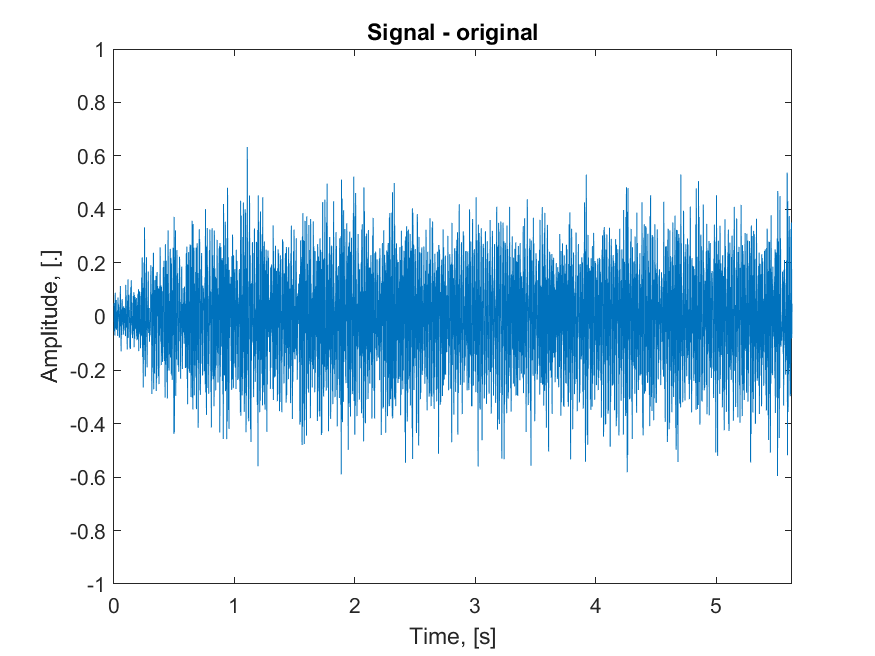
\includegraphics[width=0.5\textwidth]{task2_signal1.png}
    \caption{Изначальный график сигнала}
\end{figure}

\begin{figure}[ht]
    \centering
    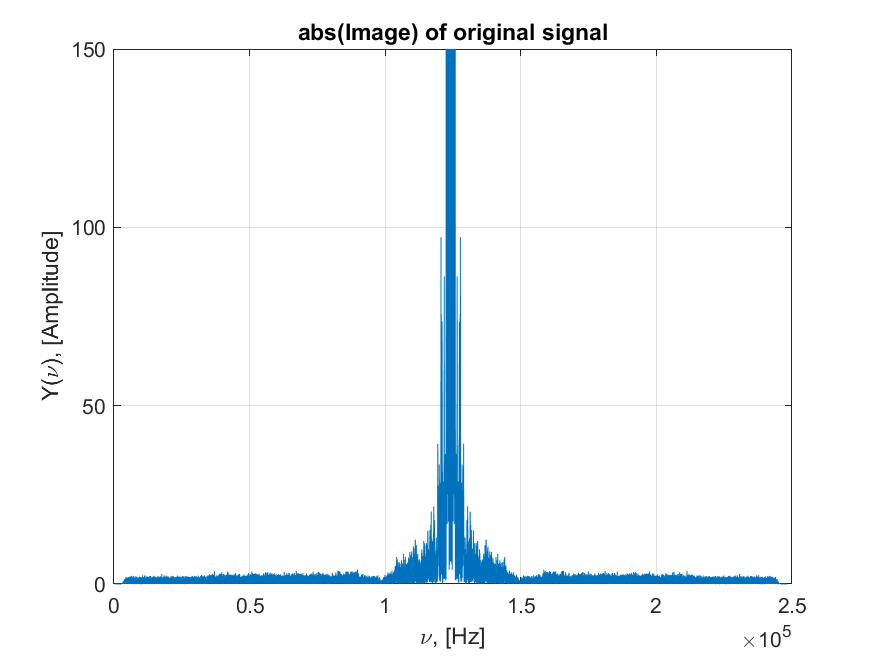
\includegraphics[width=0.5\textwidth]{task2_image1.png}
    \caption{Изначальный Фурье-образ сигнала}
\end{figure}

\begin{figure}[ht]
    \centering
    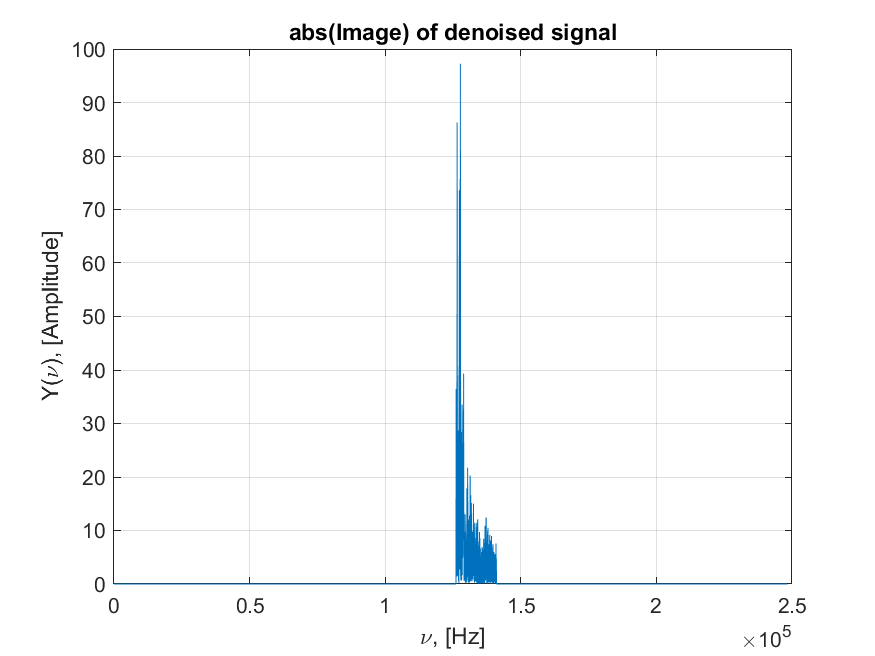
\includegraphics[width=0.5\textwidth]{task2_image2.png}
    \caption{Применили два фильтра - изменение Фурье-образа}
\end{figure}

\begin{figure}[ht]
    \centering
    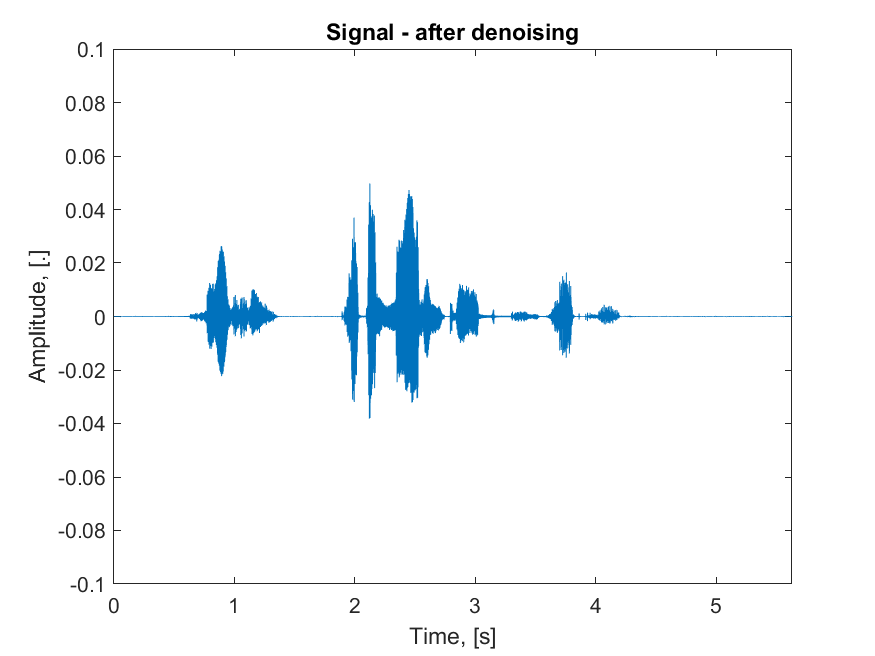
\includegraphics[width=0.5\textwidth]{task2_signal2.png}
    \caption{Очищенный вид сигнала}
\end{figure}
\newpage
 Не забывайте, что с помощью функции матлаба \texttt{sound(y,f)} - можно нативно проиграть звук после преобразований, чтобы сравнить "до" и "после".


 % \textit{NB.} - В этом задании мы используем унитарное преобразование Фурье к обычной частоте $\nu$, оно будет выглядеть следующим образом: 
% \begin{align*}
%     f(t) = \int_{-\infty}^{+\infty}\hat{f}(\nu)e^{2\pi i \nu t}dt \\
%     \hat{f}(\nu) = \int_{-\infty}^{+\infty}f(t)e^{-2\pi i \nu t}dt
% \end{align*}

% Выберем треугольную функцию и зафиксируем для неё  $a$, $b$. После рассмотрим её сдвиг $g(t) = f(t + c)$.

% \section{Фурье-образ}

% Воспользуемся хитростью, а именно свойством Фурье-оператора:
% $$
% \mathbb{F}\{f(t+\tau)\} = e^{i \omega\tau}\mathbb{F}\{f(t)\}
% $$, где $\tau$- наш сдвиг. 

% В нашем случае его можно трактовать как \textit{поворот} образа в комплексной плоскости... Поэтому образ и приобретёт комплексную гармонику.

% Образ Фурье будет выглядеть так:
% $$
% \hat{g}(\nu) = \frac{ab}{\sqrt{2\pi}}sinc^2(\frac{b\omega}{2})e^{i\omega\tau}
% $$


\endinput